\documentclass[../main]{subfiles}
\begin{document}
\section{Geometria Riemanniana}
Sobre una manifold de Riemann $(M,g)$, podemos introducir el concepto de curvatura de una manifold. En esta sección estudiaremos las bases de la geometria Riemanniana. La teoria de la Relatividad de Einstein ha sido construida en base a estos conceptos.

Hasta ahora las manifolds que hemos considerado están definidas con las nociones de derivadas e integrales. Necesitamos introducir una metrica para definir el concepto de longitud.

\definicion{(Métrica de Riemann)}. Una métrica de Riemann $g$ sobre una manifold suave $\mathcal{M}$ es una forma bilineal $g: T_p \mathcal{M}\times T_p \mathcal{M} \rightarrow \mathbb{R}$ para cualquier $p\in \mathcal{M}$ con las siguientes propiedades:
\begin{enumerate}
    \item[$(i)$] Simétrico: $g(X_p, Y_p)=g(Y_p, X_p) \ \forall \ X_p, Y_p \in T_p\mathcal{M}$.
    \item[$(ii)$] Definido-positivo: $g(X_p, Y_p)\geq 0 \ \forall \ X_p \in T_p \mathcal{M}$. 
    \item[$(iii)$] No degenerado: $g(X_p, X_p)=0$ si y solo si $X_p=0$.  
\end{enumerate}

Además, $g$ es suave en el sentido que para cualquier campo vectorial suave $X$ y $Y$ la función $x\rightarrow g_p(X_p, Y_p)$ es suave.

\proposicion{(Existencia de métricas de Riemann)} Toda manifold suave admite una métrica de Riemann.

Prueba: Sea $\{(U_{\alpha}, \varphi_{\alpha})\}$ covering charts de $\mathcal{M}$. En cada dominio de coordenadas, existe una métrica $g_{\alpha}$ dada por la métrica Euclideana $\delta_{ij}\mathrm{d}x^{i}\mathrm{d}x^{j}$ en coordenadas locales. Ahora, sea $\{\psi_{\alpha}\}$ una partición de unidad suave subordinada al cover $\{U_{\alpha}\}$ y definimos
\begin{equation}
    g=\sum_{\alpha}\psi_{\alpha}g_{a}
\end{equation}
gracias a la condición local de finitud para partición de unidades, existe solamente un número finito en un vecindario para cada punto. Así esta expresión define un campo tensorial suave. Es simétrico, así que solamente se necesita comprobar que sea definido positivo. 

Si $x \in T_p\mathcal{M}$ es un vector no nulo, entonces
\begin{equation}
    g(x, x)=\sum_{\alpha} \psi_{\alpha}(p) g_{\alpha}(x, x)\Big{|}_p
\end{equation}
esta suma no es negativa ya que $g\Big{|}_{\alpha}(x, x)>0 \ \rightarrow \ g_p(x, x)>0$.

En física, usamos como manifold pseudo-Riemannianas y usualmente no está definida positiva y el número de autovalores negativos es llamado signatura
\begin{equation}
    \mathbb{R}^{1, 3}=
    \begin{pmatrix}
        -1 & 0 & 0 & 0 \\
        0 & +1 & 0 & 0 \\
        0 & 0 & +1 & 0 \\
        0 & 0 & 0 & +1 
    \end{pmatrix}
    =
    \begin{pmatrix}
        +1 & 0 & 0 & 0 \\
        0 & -1 & 0 & 0 \\
        0 & 0 & -1 & 0 \\
        0 & 0 & 0 & -1 
    \end{pmatrix}
\end{equation}

Para un mapa suave $f:\mathcal{M}\rightarrow \mathcal{N}$, la métrica $g$ sobre una manifold $\mathcal{N}$ puede ser pull-back a la métrica $f^* g$ sobre $\mathcal{M}$ de tal manera que para $X_p, Y_p \in T_p \mathcal{M}$
\begin{equation}
    f^* g(X_p, Y_p)=g(f^* X_p, f^* Y_p)
\end{equation}

\section{Visión General}

\section{Derivada Covariante}
Consideremos 
\begin{equation}
    \begin{split}
        \partial_{\lambda'}T^{\mu'}=\pdv{T^{\mu'}}{x^{\partial_{\lambda'}}}&=\pdv{x^{\sigma}}{x^{\lambda'}}\pdv{}{x^{\sigma}}\left(\pdv{x^{\mu'}}{x^{\nu}}T^{\nu}(x)\right)\\
        &=\pdv{x^{\sigma}}{x^{\lambda'}}\pdv{x^{\mu'}}{x^{\nu}}\partial_{\sigma} T^{\nu}+\underbrace{\left(\pdv{x^{\sigma}}{x^{\lambda'}}\pdv{^2 x^{\mu}}{x^{\sigma}\partial x^{\nu}}\right)}_{\text{no tensorial}} T^{\nu}
    \end{split}
\end{equation}

Encontremos una nueva ``derivada covariante'', $\nabla_{\lambda}T^{\mu}$, que transforma como un tensor:
\begin{equation}
    \nabla_{\lambda'}T^{\mu'}=\pdv{x^{\sigma}}{x^{\lambda'}}\pdv{x^{\mu'}}{x^{\nu}}\nabla_{\sigma}T^{\nu}
\end{equation}

Sea $V$ un vector tangente a lo largo de una curva $\gamma$, la derivada covariante de un tensor a lo largo de una curva satisface:
\begin{enumerate}
    \item Linealidad: $\nabla_{V}(T+S)=\nabla_{V} T+\nabla_{V} S$.
    \item Leibniz: $\nabla_{V}(T\otimes S)=(\nabla_{V}T)\otimes S+T\otimes(\nabla_{V} S)$.
    \item Aditividad: $\nabla_{fV+gW} T=f\nabla_{V}T+g\nabla_{W}S$.
    \item Acción sobre escalares: $\nabla_V(f)=V(f)$.
    \item Acción sobre vectores: $\nabla_{\beta}e_{\alpha}=\Gamma^{\mu}_{\beta\alpha} e_{\mu}$, donde $\nabla_{\beta} \equiv \nabla_{e\beta}$.\footnote{$\Gamma^{\mu}_{\beta\alpha}$ son llamados los \textcolor{red}{coeficientes de conexión(o simbolos de Christoffel)}.}
\end{enumerate}

Sea $T=T^{\mu}e_{\mu}$ y $V=V^{\nu} e_{\nu}$. La derivada covariante de $T$ es 
\begin{equation}
    \begin{split}
        \nabla_V T=\nabla_V (T^{\mu}e_{\mu})&=\nabla_V (T^{\mu})+T^{\mu}(\nabla_V e_{\mu})\\
        &=V(T^{\mu})e_{\mu}+T^{\mu}\nabla_{V^{\nu}e_{\nu}}e_{\mu}\\
        &=V^{\nu}e_{\nu}(T^{\mu})e_{\mu}+T^{\mu}V^{\nu}\nabla_{e_{\nu}}e_{\mu}\\
        &=V^{\nu}(\partial_{\nu}T^{\mu})e_{\mu}+T^{\mu}V^{\nu}\Gamma^{\lambda}_{\nu\mu}e_{\lambda}\\
        &=V^{\nu}(\partial_{\nu}T^{\mu}+\Gamma^{\mu}_{\nu\beta}T^{\beta})e_{\mu}
    \end{split}
\end{equation}

Así las componentes resultantes de $(1, 1)$ tensor son $\nabla_{\nu} T^{\mu}=\partial_{\mu} T^{\mu}+\textcolor{red}{\Gamma^{\mu}_{\nu\lambda} T^{\lambda}}$ donde hemos definido $(\nabla T)^{\mu}_{\nu}:=\nabla_{\nu} T^{\mu}$.

Ahora, bajo una transformación de coordenadas, tenemos:
\begin{equation}
    \begin{split}
        \nabla_{\mu'}T^{\nu'}&=\partial_{\mu'}T^{\nu'}+\Gamma^{\nu'}_{\mu'\alpha'}T^{\alpha'}\\
        &=\pdv{x^{\mu}}{x^{\mu'}}\partial_{\mu}\left(\pdv{x^{\nu'}}{x^{\nu}}T^{\nu}\right)+\Gamma^{\nu'}_{\mu'\alpha'}\pdv{x^{\alpha'}}{x^{\alpha}} T^{\alpha} \\
        &=\pdv{x^{\mu}}{x^{\mu'}}\pdv{x^{\nu'}}{x^{\nu}} \partial_{\mu}T^{\nu}+\pdv{x^{\mu}}{x^{\mu'}}\pdv{x^{\nu'}}{x^{\mu}}{x^{\nu}} T^{\nu}+\Gamma^{\nu'}_{\mu'\alpha'}\pdv{x^{\alpha'}}{x^{\alpha}} T^{\alpha} \\
        &=\textcolor{blue}{\pdv{x^{\mu}}{x^{\mu'}}\pdv{x^{\nu'}}{x^{\nu}}\nabla_{\mu}T^{\nu}} \textcolor{red}{\underbrace{\left(\pdv{x^{\mu}}{x^{\mu'}}\pdv{x^{\nu'}}{x^{\nu}}\Gamma^{\nu}_{\mu\alpha}-\pdv{x^{\mu}}{x^{\mu'}}\pdv{x^{\nu'}}{x^{\mu}}{x^{\alpha}}-\Gamma^{\nu'}_{\mu'\alpha'}\pdv{x^{\alpha'}}{x^{\alpha}}\right)}_{0}T^{\alpha}}
    \end{split}
\end{equation}
usando $\partial_{\mu}T^{\nu}=\partial_{\mu} T^{\nu}-\Gamma^{\nu}_{\mu\alpha}T^{\alpha}$.

$\nabla_{\mu}T^{\mu}$ es un tensor si:
\begin{equation}
    \Gamma^{\nu'}_{\mu'\alpha'}=\textcolor{blue}{\pdv{x^{\mu}}{x^{\mu'}}\pdv{x^{\nu'}}{x^{\nu}}\pdv{x^{\alpha}}{x^{\alpha'}}\Gamma^{\nu}_{\mu\nu}}-\textcolor{red}{\pdv{x^{\mu}}{x^{\mu'}}\pdv{x^{\alpha}}{x^{\alpha'}}\pdv{x^{\nu'}}{x^{\mu}}{x^{\alpha}}}
\end{equation}

Por lo tanto $\Gamma^{\nu}_{\mu\alpha}$ no son las componentes de un $(1, 2)$ tensor.

\subsection{Derivada covariante de un co-vector}

Consideremos $f\equiv w_{\nu}T^{\nu}$ ya que $\nabla_{\mu}f=\partial_{\mu} f$, tenemos 
\begin{equation}
    \nabla_{\mu}(w_{\nu}T^{\nu})=\partial_{\mu}(w_{\nu}T^{\nu})=(\partial_{\mu}w_{\nu})T^{\nu}+w_{\nu}(\partial_{\mu}T^{\nu})
\end{equation}
o también
\begin{equation}
    \begin{split}
        \nabla_{\mu}(w_{\nu}T^{\nu})&=(\nabla_{\mu}w_{\nu})T^{\nu}+w_{\nu}(\nabla_{\mu}T^{\nu})\\
        &=(\nabla_{\mu}w_{\nu})T^{\nu}+w_{\nu}(\partial_{\mu}T^{\nu}+\Gamma^{\nu}_{\mu\alpha}T^{\alpha})
    \end{split}
\end{equation}

Comparando estas ecuaciones, obtenemos
\begin{equation}
    (\nabla_{\mu} w_{\nu})T^{\nu}=(\partial_{\mu} w_{\nu}-\Gamma^{\alpha}_{\mu\nu}w_{\alpha})T^{\nu}
\end{equation}
tal que,
\begin{equation}
    \nabla_{\mu} w_{\nu}=\partial_{\mu} w_{\nu}-\textcolor{red}{\Gamma^{\alpha}_{\mu\nu}w_{\alpha}}
\end{equation}

Esto generaliza a tensores arbitrarios, por ejemplo 
\begin{equation}
    \nabla_{\mu} T^{\gamma}_{\alpha\beta}=\partial_{\mu} T_{\alpha\beta}^{\gamma}+\textcolor{blue}{\Gamma^{\gamma}_{\mu\lambda} T^{\lambda}_{\alpha\beta}}-\textcolor{red}{\Gamma^{\lambda}_{\mu\alpha}T^{\gamma}_{\lambda\beta}-\Gamma^{\lambda}_{\mu\beta}T^{\lambda}_{\alpha\beta}}
\end{equation}
hasta ahora no hemos usado el tensor métrico para definir $\nabla$.

\definicion{(Conexión).} Sea $X$ y $Y$ campos vectoriales sobre $\mathcal{M}$. El símbolo $\nabla_{\alpha} Y$ denota la derivada del campo vectorial $Y$ a lo largo del flujo del campo vectorial $X$. De hecho, $\nabla$ es un mapa:
\begin{equation}
    \begin{split}
        \nabla: &\mathfrak{X}(\mathcal{M}) \times \mathfrak{X}(\mathcal{M}) \rightarrow \mathfrak{X}(\mathcal{M})\\
        &(X, Y) \rightarrow \nabla_X Y
    \end{split}
\end{equation}
el cual satisface las siguientes condiciones:
\begin{enumerate}
    \item $\nabla$ es linear en la primera variable y aditiva en la segunda:
    \begin{align}
        \nabla_{fX+hY}Z&=f\nabla_X Z+h\nabla_Y Z\\
        \nabla_X (Y+Z)&=\nabla_X Y+\nabla_X Z
    \end{align}
    donde $f, h\in \mathbb{C}^{\infty}(\mathcal{M})$ son funciones y $X, Y, Z \in \mathfrak{X}(\mathcal{M})$ son campos vectoriales.
    \item $\nabla$ obedece la regla de Leibniz en la segunda variable 
    \begin{equation}
        \nabla_X (fY)=X(f)Y+f\nabla_X Y.
    \end{equation}
    El operador $\nabla$ es llamado conexión.
\end{enumerate}
Existe un número infinito de conexiones sobre una manifold $\mathcal{M}$. Sin embargo, dada una métrica de Riemann $g$ en $\mathcal{M}$, hay una elección natural para la conexión, el cual es llamada la \textcolor{red}{conexión de Levi-Civita.}

\definicion{(Conexión de Levi-Civita).} La conexión de Levi-Civita es la conexión única tal que:
\begin{enumerate}
    \item Libre de Torsión: $T^{\alpha}_{\mu\nu}\equiv \Gamma^{\alpha}_{\mu\nu}-\Gamma^{\alpha}_{\nu\mu}=0$.
    \item Compatible ocn la métrica: $\nabla_{\lambda} g_{\mu\nu}=0$.
\end{enumerate}

Vamos a construir la conexión de Levi-Civita escribiendo $\nabla_{\lambda}g_{\mu\nu}=0$ tres veces 
\begin{align}
    \nabla_{\lambda}g_{\mu\nu}&=\partial_{\lambda}g_{\mu\nu}-\textcolor{red}{\Gamma^{\sigma}_{\lambda\mu}g_{\sigma\nu}}-\textcolor{blue}{\Gamma^{\sigma}_{\lambda\nu}g_{\mu\sigma}}=0 \tag{$a$} \label{eca}\\
    \nabla_{\mu}g_{\nu\lambda}&=\partial_{\mu}g_{\nu\lambda}-\textcolor{brown}{\Gamma^{\sigma}_{\mu\nu}g_{\sigma\lambda}}-\textcolor{red}{\Gamma^{\sigma}_{\mu\lambda}g_{\nu\sigma}}=0 \tag{$b$} \label{ecb}\\
    \nabla_{\nu}g_{\lambda\mu}&=\partial_{\nu}g_{\lambda\mu}-\textcolor{blue}{\Gamma^{\sigma}_{\nu\lambda}g_{\sigma\mu}}-\textcolor{brown}{\Gamma^{\sigma}_{\nu\mu}g_{\lambda\sigma}}=0 \tag{$c$} \label{ecc}
\end{align}
usando \eqref{eca}-\eqref{ecb}-\eqref{ecc} dará: 
\begin{equation}
    \partial_{\lambda}g_{\mu\nu}-\partial_{\mu}g_{\nu\lambda}-\partial_{\nu}g_{\lambda\mu}+\textcolor{brown}{2\Gamma^{\sigma}_{\mu\nu}g_{\sigma\lambda}}=0 \ \rightarrow \ \Gamma^{\alpha}_{\mu\nu}=\dfrac{1}{2}g^{\alpha\lambda}\left(\partial_{\mu} g_{\nu\lambda}+\partial_{\nu} g_{\lambda\mu}-\partial_{\lambda}g_{\mu\nu}\right) 
\end{equation}

\textcolor{red}{Nota:} De espacio-tiempo plano a curvos\\

Ecuaciones relativistas deben ser construidas con derivadas covariantes, no derivadas parciales, así de Relatividad Especial a Relatividad General: $\partial_{\mu} \rightarrow \nabla_{\mu}$.

Ejemplo:
\begin{equation}
    \begin{split}
        \partial_{\nu} F^{\mu\nu}=J^{\mu} \ &\rightarrow \ \nabla_{\mu}F^{\mu\nu}=J^{\mu}\\
        \partial_{\nu} T^{\mu\nu}=0 \ &\rightarrow \ \nabla_{\nu} T^{\mu\nu}=0
    \end{split}
\end{equation}

\section{Transporte paralelo y Geodesicas}

Dada una conexión $\nabla$ sobre un bundle vectorial $E$, podemos definir direcciones \textcolor{red}{horizontal} en el espacio $\Gamma(E)$ de secciones. Una sección $s \in \Gamma(E)$ es \textcolor{red}{paralela} a lo largo de un camino $\gamma: I \rightarrow \mathcal{M}$:
\begin{equation}
    \nabla_{\dot{\gamma}(t)}s=0 \quad \text{para} \quad t\in I
\end{equation}

En coordenadas locales, puede ser escrito como:
\begin{equation}
    \dv{s_i}{t}+\sum_{j=1}^n s_j(A_{\mu})^j_i \dv{x^{\mu}}{t}=0
\end{equation}

Un teorema de ecuaciones diferenciales ordinarias, nos dice que dada unas condiciones iniciales $S(t=0) \in E_{\gamma(0)}$ podemos transportar paralelamente a lo largo de $\gamma(t)$ así tenemos el mapa 
\begin{equation}
    E_{\gamma(0)} \ni s(t=0) \ \rightarrow \ S(t=1) \in E_{\gamma(1)}
\end{equation}

En particular, si consideramos una curva $p=\gamma(0)=\gamma(1)$, obtenemos un mapa $\tau_{\gamma}: E_p \rightarrow E_p$. Para dos curvas dadas $\gamma_1, \gamma_2$ podemos tener una multiplicación $\tau_{\gamma_1 \circ \gamma_2}=\tau_{\gamma_1}\circ \tau_{\gamma_2}$ y la inversa es definida por $\tau_{\gamma^{-1}}=\tau^{-1}_{\gamma}$, tal que forme un grupo llamado grupo de homología.

En geometría euclideana, las lineas paralelas se mantienen paralelas ¿Cómo se generaliza esto a espacios curvos?

En espacio-tiempo plano, el \textcolor{red}{transporte paralelo} de un vector $v^{\mu}$ a lo largo de una curva $x^{\mu}(\lambda)$ significa 
\begin{equation}
    \dv{v^{\mu}}{\lambda}=\dv{x^{\mu}}{\lambda}\partial_{\nu}v^{\mu}=0 \quad (\text{espacio-tiempo plano})
\end{equation}

Así podemos generalizarlo a espacio-tiempo curvo, si $\partial \rightarrow \nabla$:
\begin{equation}
    \begin{split}
        \dfrac{D v^{\mu}}{D\lambda}=\dv{x^{\mu}}{\lambda}\nabla_{\nu}v^{\mu}&=0 \quad (\text{espacio-tiempo curvo})\\
        \dv{v^{\mu}}{\lambda}+\Gamma^{\mu}_{\sigma\nu}\dv{x^{\sigma}}{\lambda}v^{\nu}&=0
    \end{split}
\end{equation}
donde $\Gamma^{\mu}_{\sigma\nu}$ determina como las componentes de un vector cambian a lo largo de una curva.

Una \textcolor{red}{geodésica} es una curva a lo largo de la cual el vector tangente $\dv{x^{\mu}}{\lambda}$ se transporta en paralelo 
\begin{equation}
    v^{\mu}=\dv{x^{\mu}}{\lambda} \ \rightarrow \ v^{\mu}\nabla_{\nu}v^{\mu}=0 \ \rightarrow \ \dv{^2 x^{\mu}}{\lambda^2}+\Gamma^{\mu}_{\sigma\lambda}\dv{x^{\sigma}}{\lambda}\dv{x^{\nu}}{\lambda}=0
\end{equation}

La cual es igual a la \textcolor{red}{ecuación de la geodésica} si identificamos $\Gamma^{\mu}_{\sigma\nu}$ con las conexiones de Levi-Civita.

\section{Simetrías y vectores de Killing}

Un campo vectorial $X$ sobre una manifold Riemanniana ($\mathcal{M}, g$) es llamado \textcolor{red}{campos vectoriales de Killing} si su flujo se convierte $\varphi^*_1 g=g$, osu derivada de la métrica $g$ se anula
\begin{equation}
    \mathcal{L}_X g=0
\end{equation}
Si escribimos la métrica $\mathrm{d}s^2=g_{ij}\mathrm{d}x^{i}\mathrm{d}x^j$ y el campo vectorial de Killing $X=X^k\partial_{k}$ en términos de una coordenada local $(u; x^1, \cdots, x^n)$, la ecuación de campo de Killing puede ser escrita como 
\begin{equation}
    X^k \partial_k g_{ij}+g_{kj}\partial_i X^k+g_{ik}\partial_j X^k=0
\end{equation}

Usando una métrica $g$, tenemos un isomorfismo entre el campo vectorial y 1-forma 
\begin{equation}
    \hat{g}: \mathfrak{X}(\mathcal{M}) \cong \Omega^1(\mathcal{M})
\end{equation}
de manera que para los campos vectoriales $X, Y \in \mathfrak{X}(\mathcal{M})$ sobre $\mathcal{M}$, $\hat{g}(X)(Y)=g(X, Y)$.

Usando el isomorfismo $T_p \mathcal{M} \cong T^*_p \mathcal{M}$, podemos introducir un producto interno sobre $T^*_p\mathcal{M}$.

Consideremos $x^{\mu} \rightarrow \tilde{x}^{\mu}(x)$ como una transformación \textcolor{red}{activa} entre diferentes puntos en la manifold. Puntos vecinos estarán conectados por transformaciones infinitesimales
\begin{equation}
    \begin{split}
        x^{\mu} \rightarrow \tilde{x}^{\mu}(x)&=x^{\mu}+\delta x^{\mu}\\
        &=x^{\mu}-v^{\mu}
    \end{split}
\end{equation} 

\proposicion{} La métrica cambia como $\delta g_{\mu\nu}=\nabla_{\mu} v_{\nu}+\nabla_{\nu} v_{\mu}$.

Proof: Recordemos que 
\begin{equation}
    g_{\mu\nu}(x) \rightarrow \tilde{g}_{\mu\nu}(\tilde{x}) = \pdv{x^{\rho}}{\tilde{x}^{\mu}} \pdv{x^{\lambda}}{\tilde{x}^{\nu}}g_{\rho\lambda}(x),
\end{equation}
donde 
\begin{equation}
    \pdv{\tilde{x}^{\mu}}{x^{\rho}}=\delta^{\mu}_{\rho}-\partial_{\rho} v^{\mu} \ \rightarrow \ \pdv{x^{\rho}}{\tilde{x}^{\mu}}=\delta^{\rho}_{\mu}+\partial_{\mu}v^{\rho}
\end{equation}

Así, obtenemos 
\begin{equation}
    \begin{split}
        \tilde{g}_{\mu\nu}(\tilde{x})&=\left(\delta^{\rho}_{\mu}+\partial_{\mu}v^{\rho}\right)\left(\delta^{\lambda}_{\nu}+\partial_{\nu}v^{\lambda}\right)g_{\rho\lambda}(x)\\
        &=g_{\mu\nu}(x)+\partial_{\mu}v^{\rho}g_{\rho\nu}(x)+\partial_{\nu}v^{\lambda}g_{\mu\lambda}(x)
    \end{split}
\end{equation}

Escribiendo 
\begin{equation}
    g_{\mu\nu}(x)=g_{\mu\nu}(\tilde{x}+v)=g_{\mu\nu}(\tilde{x})+v^{\lambda}\partial_{\lambda} g_{\mu\nu}(x),
\end{equation}
obtenemos:
\begin{equation}
    \begin{split}
        \delta g_{\mu\nu}&=\tilde{g}_{\mu\nu}(\tilde{x})-g_{\mu\nu}(\tilde{x})\\
        &=v^{\lambda}\partial_{\lambda} g_{\mu\nu}+\partial_{\mu}v^{\rho}g_{\rho\nu}+\partial_{\nu}v^{\lambda}g_{\mu\lambda}\\
        &=v^{\lambda}\partial_{\lambda} g_{\mu\nu}+\partial_{\mu}(v^{\rho}g_{\rho\nu})+\partial_{\nu}(v^{\lambda}g_{\mu\lambda})-v^{\rho}\partial_{\mu} g_{\rho\nu}-v^{\lambda} \partial_{\nu}g_{\mu\lambda}\\
        &=\nabla_{\mu} v_{\nu}+\nabla_{\nu}v_{\mu}+\Gamma^{\alpha}_{\mu\nu}v_{\alpha}+\Gamma^{\alpha}_{\nu\mu}v_{\alpha}-v^{\lambda}(\partial_{\mu}g_{\nu\lambda}+\partial_{\nu}g_{\mu\lambda}-\partial_{\lambda}g_{\mu\nu})\\
        &=\nabla_{\mu} v_{\nu}+\nabla_{\nu}v_{\mu}. \quad \square 
    \end{split}
\end{equation}

Para una \textcolor{red}{transformación de simetría}, tenemos $\delta g_{\mu\nu}=0 \ \rightarrow \ \nabla_{\mu} v_{\nu}+\nabla_{\nu} v_{\mu}=0$ (\textcolor{red}{ecuación de Killing}), donde $v^{\mu}$ es un \textcolor{red}{vector de Killing}. Encontrar todos los vectores de Killing de una métrica $g_{\mu\nu}$ puede ser difícil, algunas propiedades son:
\begin{itemize}
    \item Si $\partial_{\alpha} g_{\mu\nu}=0$, entonces $\partial_{\alpha}$ es un vector de Killing.
    \item Si $K$ y $Z$ son vectores de Killing, entonces $\alpha K+\beta Z$ es un vector de Killing.
    \item Si $K$ y $Z$ son vectores de Killing, entonces $[K, Z]$ es un vector de Killing.
\end{itemize}  

\ejemplo{} Consideremos $\mathbb{R}: \mathrm{d}x^2+\mathrm{d}y^2+\mathrm{d}z^2$.

Tres vectores de Killing son $x=\partial_x$, $y=\partial_y$ y $z=\partial_z$ con componentes:
\begin{equation}
    \left.
    \begin{array}{c}
        x^{\mu}=(1, 0, 0)\\
        y^{\mu}=(0, 1, 0)\\
        z^{\mu}=(0, 0, 1)
    \end{array}
    \right\}
    \leftarrow \ \text{Translaciones a lo largo de } x, y, z
\end{equation}
Cambiando a coordenadas polares:
\begin{equation}
    \left\{
    \begin{array}{c}
        x= r\sin \theta \cos \phi \\
        y= r\sin \theta \sin \phi \\
        z= r\cos \theta
    \end{array}
    \right.
\end{equation}

Obtenemos 
\begin{equation}
    \mathrm{d}s^2=\mathrm{d}r^2+r^2\mathrm{d}\theta^2+r^2\sin^2 \theta \mathrm{d}\phi^2
\end{equation}
otro vector de Killing es 
\begin{equation}
    R=\partial_{\phi}=-y\partial_x+x\partial_y \ \rightarrow \ R^{\mu}=(-y, x, 0)
\end{equation}

Permutando coordenadas, obtenemos 
\begin{equation}
    \left.
    \begin{array}{c}
        R^{\mu}=(-y, x, 0)\\
        S^{\mu}=(z, 0, -x)\\
        T^{\mu}=(0, -z, y)
    \end{array}
    \right\}
    \leftarrow \ \text{rotaciones alrededor de } z, y, x
\end{equation}

\textcolor{blue}{Teorema de Noether:} 
\begin{center}
    Simetrías \ $\rightarrow$ \ Cantidades conservadas.
\end{center}

\proposicion{} Consideremos una geodésica con vector tangente $P^{\mu}=\mathrm{d}x^{\mu}/\mathrm{d}\lambda$. Así $Q=K^{\mu}P_{\mu}$ es conservada a lo larga de la geodésica.

Proof: Consideremos la derivada direccional de $Q$:
\begin{equation}
    \begin{split}
        \dfrac{D(K^{\nu}P_{\nu})}{D\lambda}&= P^{\mu}\nabla_{\mu}(K^{\nu}P_{\nu})=P^{\mu}P^{\nu}\nabla_{\mu}K_{\nu}+(P^{\mu}\nabla_{\mu}P^{\nu})K_{\nu}\\
        &=\dfrac{1}{2}P^{\mu}P^{\nu}(\nabla_{\mu}K_{\nu}+\nabla_{\nu}K_{\mu})=0. \quad \square
    \end{split}
\end{equation}

\ejemplo{}
\begin{itemize}
    \item Traslaciones de tiempo $K=\partial_t$, $Q=K^{\mu}P_{\mu}=P_0$ (Energía).
    \item Traslaciones espaciales $K=\partial_i$, $Q=K^{\mu}P_{\mu}=P_i$ (Momentum).
    \item Rotaciones $K=\partial_{\phi}$, $Q=K^{\mu}P_{\mu}=P_{\phi}$ (Momento angular).
\end{itemize}

Sea $(u, \{x^{i}\})$ coordenadas locales sobre $\mathcal{M}$. Ya que $\nabla_{\pdv{}{x^{i}}} \pdv{}{x^{k}}$ es un campo vectorial, puede ser expresado como una combinación lineal de los campos ordenados sobre $u$:
\begin{equation}
    \nabla_{\pdv{}{x^{i}}} \pdv{}{x^k}:= \Gamma^{i}_{jk} \pdv{}{x^{i}},
\end{equation}
donde $\Gamma^{i}_{jk}$ son llamados los \textcolor{red}{Simbolos de Christoffel}. Si escribimos el campo vectorial $X=x^{i}\pdv{}{x^{i}}$, $Y=y^{i}\pdv{}{x^{i}}$ en términos de estas bases, entonces la derivada covariante es expresada como 
\begin{equation}
    \nabla_x Y=X^{i}\left(\pdv{Y^k}{x^{i}}+\Gamma^{\alpha}_{\ij} Y^j\right)\pdv{}{x^k}
\end{equation}

Sea $\gamma: I \rightarrow \mathcal{M}$ una curva sobre $\mathcal{M}$ y definimos:
\begin{equation}
    J(\gamma)=\{ \text{Campos vectoriales a lo largo de } \gamma \}
\end{equation}

Entonces, dada la conexión $\nabla$, podemos definir la \textcolor{red}{derivada covariante} a lo largo de $\gamma$, el cual es un mapa 
\begin{equation}
    \dfrac{\mathrm{D}}{\mathrm{d}t}: J(\gamma)\rightarrow J(\gamma) \ \text{tal que:}
\end{equation}
\begin{enumerate}
    \item[$(i)$] $\displaystyle \dfrac{\mathrm{D} (x+y)}{\mathrm{d}t}=\dfrac{\mathrm{D}x}{\mathrm{d}t}+\dfrac{\mathrm{D}y}{\mathrm{d}t}$.
    \item[$(ii)$] $\displaystyle \dfrac{\mathrm{D}(fx)}{\mathrm{d}t}=\dv{f}{t}x+f\dfrac{\mathrm{D}x}{\mathrm{d}t} \ \forall \ f\in C^{\infty}(I)$.
    \item[$(iii)$] Si $x \in J(\gamma)$ es inducido por un campo vectorial $\displaystyle \tilde{x}\left(\tilde{x}\Big{|}_{\gamma(t)}=x(t) \ \forall \ t\in I\right)$ entonces, $\displaystyle \dfrac{\mathrm{D}x}{\mathrm{d}t}\Big{|}_{t=0}=\nabla_{\dot{\gamma}(0)}\tilde{x}$.   
\end{enumerate}

En términos de coordenadas locales, podemos escribirlo como:
\begin{equation}
    \dfrac{\mathrm{D}x}{\mathrm{d}t}=\left(\dv{x^k}{t}+\Gamma^k_{ij}\dv{x^{i}}{t}x^j\right)\pdv{}{x^k},
\end{equation}
donde $\gamma(t)=(x^1(t), \cdots, x^n(t))$.

Dado un camino $\gamma(t)$(no necesariamente una geodésica), un campo vectorial $X$ es llamado \textcolor{red}{campo vectorial paralelo} a lo largo de $\gamma$ si:
\begin{equation}
    \dfrac{\mathrm{D}X}{\mathrm{d}t}=0.
\end{equation}

Los símbolos de Christoffel $\Gamma^k_{ij}$, el camino $\gamma$, y las derivadas $\dv{x^{i}}{t}$ son conocidos. Entonces, en un sistema de $n$ ecuaciones diferenciales lineales de primer orden en términos de coordenadas locales:
\begin{equation}
    \dv{x^k}{t}+\Gamma^k_{ij}x^j \dv{x^{i}}{t}=0 \quad \text{para} \ k=1, \cdots, n.
\end{equation}

Ya que esto es un conjunto de ecuaciones diferenciales, existe así una única solución $x(t)$ dada las condiciones iniciales $x(0) \in T_{\gamma(0)}\mathcal{M}$. El vector $x(t)$ es obtenido de $x(0)$ por \textcolor{red}{transporte paralelo} a lo largo de la curva $\gamma$:

\begin{minipage}{0.5\textwidth}
    Consideremos un paralelogramo infinitesimal 
    \\
    \begin{center}
        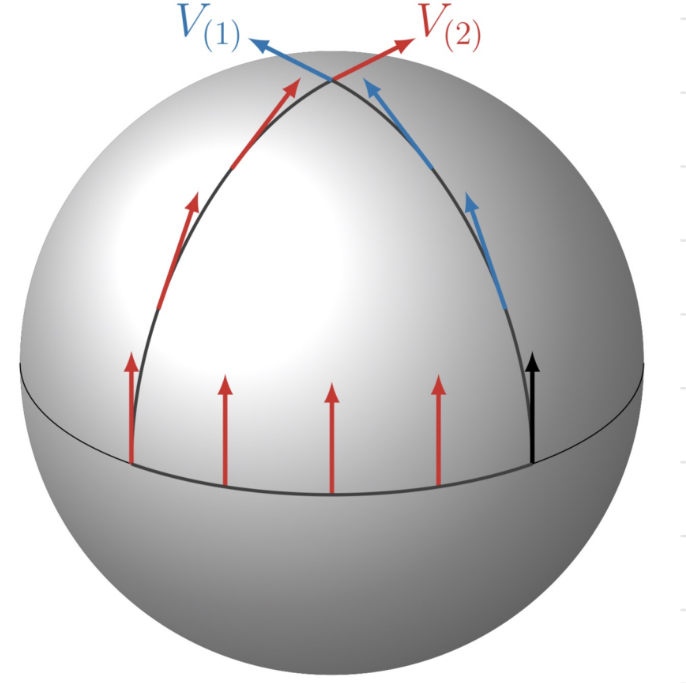
\includegraphics[scale=0.4]{img/imgRG4.2.PNG}
    \end{center}
\end{minipage}
\begin{minipage}{0.5\textwidth}
    \begin{center}
        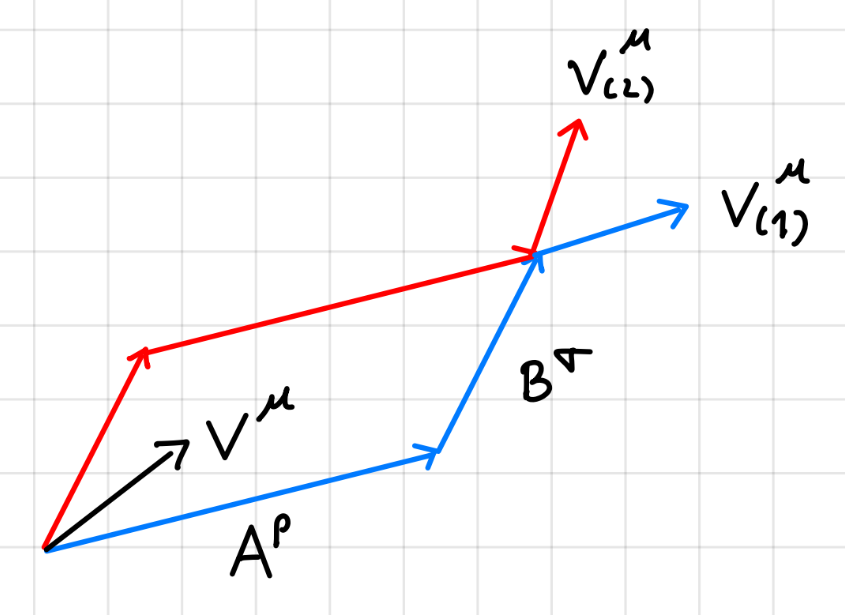
\includegraphics[scale=0.4]{img/imgRG4.3.PNG}
    \end{center}
\end{minipage}

El cambio del vector a lo largo de un lado $\delta x^{\rho}$ es:
\begin{equation}
    \begin{split}
        \delta V^{\mu}&=\dv{V^{\mu}}{\lambda}\delta \lambda = -\Gamma^{\mu}_{\nu\rho} V^{\nu} \dv{x^{\rho}}{\lambda} \delta \lambda \quad \text{usando} \quad \dfrac{\mathrm{D}V^{\mu}}{\mathrm{D}\lambda}=\dv{V^{\mu}}{\lambda}+\Gamma^{\mu}_{\nu\rho}V^{\nu}\dv{x^{\rho}}{\lambda}\delta\lambda=0\\
        &=-\Gamma^{\mu}_{\nu\rho}V^{\nu}\delta x^{\rho}.
    \end{split}
\end{equation}

El transporte paralelo a lo largo de dos caminos da:
\begin{align}
    \textcolor{blue}{\delta V^{\mu}_{(1)}}&=-\Gamma^{\mu}_{\nu\rho}(x)V^{\nu}(x)A^{\rho}-\Gamma^{\mu}_{\nu\rho}(x+A)V^{\nu}(x+A)B^{\rho},\\
    \textcolor{red}{\delta V^{\mu}_{{(2)}}}&=-\Gamma^{\mu}_{\nu\rho}(x)V^{\nu}(x)B^{\rho}-\Gamma^{\mu}_{\nu\rho}(x+B)V^{\nu}(x+B)A^{\rho}.
\end{align}

La diferencia es 
\begin{equation}
    \begin{split}
        \delta V^{\mu} &= \delta V^{\mu}_{(1)}-\delta V^{\mu}_{(2)}\\
        &=\partial_{\sigma}\left(\Gamma^{\mu}_{\nu\rho}V^{\nu}\right)B^{\sigma}A^{\rho}-\partial_{\sigma}(\Gamma^{\mu}_{\nu\rho}V^{\nu})A^{\sigma}B^{\rho}+\cdots \\
        &=\left(\partial_{\sigma}\Gamma^{\mu}_{\nu\rho}V^{\nu}+\Gamma^{\mu}_{\nu\rho}\partial_{\sigma}V^{\nu}-\partial_{\rho}\Gamma^{\mu}_{\nu\sigma}V^{\nu}-\Gamma^{\mu}_{\nu\sigma}\partial_{\rho}V^{\nu}\right)A^{\rho}B^{\sigma}
    \end{split}
\end{equation}

Usando $\partial_{\sigma}V^{\nu}=-\Gamma^{\nu}_{\sigma\lambda}V^{\lambda}$ tenemos:
\begin{equation}
    \delta V^{\mu}=R^{\mu}_{\nu\rho\sigma}A^{\rho}B^{\sigma}V^{\nu}
\end{equation}

Donde definimos el \textcolor{red}{tensor de Riemann} como:
\begin{equation}
    R^{\mu}_{\nu\rho\sigma}=\partial_{\rho}\Gamma^{\mu}_{\nu\sigma}-\partial_{\sigma}\Gamma^{\mu}_{\nu\rho}+\Gamma^{\mu}_{\rho\lambda}\Gamma^{\lambda}_{\nu\sigma}-\Gamma^{\mu}_{\sigma\lambda}\Gamma^{\lambda}_{\nu\rho}.
\end{equation}

Por otra parte, consideremos:
\begin{equation}
    \begin{split}
        [\nabla_{\mu}, \nabla_{\nu}]V^{\rho}&=\nabla_{\mu}\nabla_{\nu} V^{\rho}-\nabla_{\nu}\nabla_{\mu}V^{\rho}\\
        &=\partial_{\mu}(\nabla_{\nu}V^{\rho})-\Gamma^{\lambda}_{\mu\nu}\nabla_{\lambda}V^{\rho}+\Gamma^{\rho}_{\mu\sigma}\nabla_{\nu}V^{\sigma}-(\mu \leftrightarrow \nu)\\
        &=\partial_{\mu}\partial_{\nu}V^{\rho}+(\partial_{\mu}\Gamma^{\rho}_{\nu\sigma})V^{\sigma}+\Gamma^{\rho}_{\nu\sigma}\partial_{\mu}V^{\sigma}-\Gamma^{\lambda}_{\mu\nu}\partial_{\lambda}V^{\rho}-\Gamma^{\lambda}_{\mu\nu}\Gamma^{\rho}_{\lambda\sigma}V^{\sigma}\\
        &\quad +\Gamma^{\rho}_{\mu\sigma}\partial_{\nu}V^{\sigma}+\Gamma^{\rho}_{\mu\sigma}\Gamma^{\sigma}_{\nu\lambda}V^{\lambda}-(\mu \leftrightarrow \nu)\\
        &=(\partial_{\mu}\Gamma^{\rho}_{\nu\sigma}-\partial_{\nu}\Gamma^{\rho}_{\mu\sigma}+\Gamma^{\rho}_{\mu\lambda}\Gamma^{\lambda}_{\nu\sigma}-\gamma^{\rho}_{\nu\lambda}\Gamma^{\lambda}_{\mu\sigma})V^{\sigma}-2\Gamma^{\lambda}_{\mu\nu}\nabla_{\lambda}V^{\rho}
    \end{split}
\end{equation}

Así, encontramos que:
\begin{equation}
    [\nabla_{\mu}, \nabla_{\nu}]V^{\rho}=R^{\rho}_{\sigma\mu\nu}V^{\sigma}-T^{\lambda}_{\mu\nu}\nabla_{\lambda}V^{\rho}
\end{equation}
para las conexiones de Levi-Civita, tenemos:
\begin{equation}
    [\nabla_{\mu}, \nabla_{\nu}]V^{\rho}=R^{\rho}_{\sigma\mu\nu}V^{\sigma}
\end{equation}
que se conoce como la identidad de Ricci.

\definicion{} El \textcolor{red}{tensor de torsión} es un mapa de dos campos vectoriales a un tercer campo vectorial 
\begin{equation}
    T(x, y)=\nabla_x y-\nabla_y x-[x, y].
\end{equation}

\definicion{} El \textcolor{red}{tensor de Riemann} es un mapa de tres campos vectoriales a un cuarto campo vectorial
\begin{equation}
    R(x, y)z=\nabla_x \nabla_y z-\nabla_y \nabla_x z-\nabla_{(x, y)}z.
\end{equation}

\section{Curvatura de Riemann}

\begin{minipage}{0.5\textwidth}
    Podemos considerar hacer un transporte paralelo sobre $S^n$ a lo largo del camino cerrado en contra de las agujas del reloj. 
    
    Podemos ver que luego de transportar paralelamente un vector a traves de un camino cerrado, obtenemos un vector diferente al inicial. La curvatura de Riemann es definida para medir esta diferencia. 

    El cual está parametrizado como $(t, s) \rightarrow \gamma(t, s)$. Entonces, la diferencia de dos vectores es dada por el tensor de Riemann 
    \begin{equation}
        \dfrac{\mathrm{D}}{\mathrm{d}t}\dfrac{\mathrm{D}}{\mathrm{d}s}X-\dfrac{\mathrm{D}}{\mathrm{d}s}\dfrac{\mathrm{D}}{\mathrm{d}t}X=R\left(\dv{\gamma}{t}, \dv{\gamma}{s}\right)X.
    \end{equation}
\end{minipage}
\begin{minipage}{0.5\textwidth}
    \begin{center}
        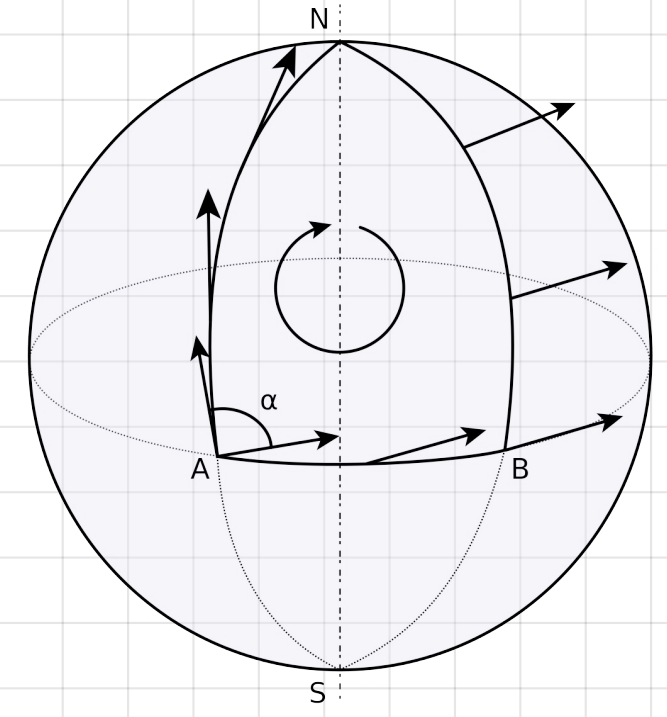
\includegraphics[scale=0.42]{img/imgRG4.4.PNG}
    \end{center}
\end{minipage}

Sea $(\mathcal{M}, g)$ una manifold de Riemann y $\nabla$ la conexión de Levi-Civita. La correspondiente curvatura es llamada el \textcolor{red}{tensor de curvatura de Riemann}, y asuimos que la curvatura es siempre el tensor de curvatura de Riemann, si introducimos la siguiente notación:
\begin{align}
    R(x, y, z, w)&:=g(R(x,y)z, w)\\
    R(\partial_x, \partial_{\ell}, \partial_j, \partial_i)&:=R_{ijk\ell}:= R^s_{jk\ell}g_{si},
\end{align}
entonces, el tensor de curvatura de Riemann satisface las siguientes propiedades:
\begin{enumerate}
    \item[$(i)$] $R(x, y, z, w)=-R(y, x, z, w)$.
    \item[$(ii)$] $R(x, y, z, w)=-R(x, y, w, z)$.
    \item[$(iii)$] $R(x, y, z, w)= R(z, w, x, y)$.
    \item[$(iv)$] $R(x, y)z+R(y, z)x+R(z, x)y=0$ (Primera identidad de Bianchi).
    \item[$(v)$] $\nabla_w R(x, y)z+\nabla_x R(y, w)z+\nabla_y R(w, x)z=0$ (Segunda identidad de Bianchi).    
\end{enumerate}

En términos de coordenadas locales, las propiedades anteriores se pueden reescribir como 
\begin{enumerate}
    \item[$(i)$] $R_{\textcolor{red}{\mu\nu}\rho\sigma}=-R_{\textcolor{red}{\nu\mu}\rho\sigma}$.
    \item[$(ii)$] $R_{\mu\nu\textcolor{blue}{\rho\sigma}}=-R_{\mu\nu\textcolor{blue}{\sigma\rho}}$.
    \item[$(iii)$] $R_{\textcolor{red}{\mu\nu}\textcolor{blue}{\rho\sigma}}=R_{\textcolor{blue}{\rho\sigma}\textcolor{red}{\mu\nu}}$.
    \item[$(iv)$] $R_{\mu\textcolor{brown}{\nu\rho\sigma}}+R_{\mu\textcolor{brown}{\rho\sigma\nu}}+R_{\mu\textcolor{brown}{\sigma\nu\rho}}=0$.
    \item[$(v)$] $\nabla_{\lambda} R_{\mu\nu\rho\sigma}+\nabla_{\nu}R_{\lambda\mu\rho\sigma}+\nabla_{\mu}R_{\nu\lambda\rho\sigma}=0$.     
\end{enumerate}

\textbf{Simetrías del tensor de Riemann:} Solo 20 de las $4^4=256$ componentes de $R^{\mu}_{\nu\rho\sigma}$ son independientes. Muchas de las componentes de $R_{\mu\nu\rho\sigma}=g_{\mu\lambda}R^{\lambda}_{\nu\rho\sigma}$ son relacionados por simetrías.

Contrayendo el primer y último índice de un tensor de curvatura de Riemann da el \textcolor{red}{tensor de curvatura de Ricci}.
\begin{equation}
    \mathrm{Ric}(g)=R_{ij}\mathrm{d}x^j \otimes \mathrm{d}x^{i}:= R^s_{ijs}=R_{kij\ell}g^{k\ell}
\end{equation}

Si existe una constante $\Lambda$ tal que $R_{ij}=\Lambda g_{ij}$, entonces $(\mathcal{M}, g)$ es llamada una \textcolor{red}{manifold de Einstein}. Contrayendo los índices de nuevo, obtenemos el \textcolor{red}{escalar de curvatura}
\begin{equation}
    R:= R_{ij} g^{ij}.
\end{equation}

\definicion{} La única contracción del tensor de Riemann es el \textcolor{red}{tensor de Riemann}
\begin{equation}
    R_{\mu\nu}=R^{\lambda}_{\mu\nu\lambda}=\partial_{\lambda}\Gamma^{\lambda}_{\mu\nu}-\partial_{\nu}\Gamma^{\lambda}_{\mu\lambda}+\Gamma^{\lambda}_{\lambda\rho}\Gamma^{\rho}_{\mu\nu}-\Gamma^{\rho}_{\mu\lambda}\Gamma^{\lambda}_{\nu\rho}.
\end{equation}

\definicion{} La traza del tensor de Ricci es el \textcolor{red}{escalar de Ricci}
\begin{equation}
    R=R^{\mu}_{\mu}=g^{\mu\nu}R_{\mu\nu}.
\end{equation}

\end{document}